\section{Numerical examples}
\label{sec:num-examples}
In this section, we present a numerical example to demonstrate the capability of the proposed model. 
%To verify the implementation, we performed several other numerical experiments in \ref{Sec:App}.
\subsection{Mandel's problem}
This example aims to study \dots
%In the sequel, we first describe how we solved Mandel's problem with our algorithm.
Consider a 2D rectangular domain of width $2a$ and height $2b$ occupied by a saturated poroelastic material. Constant compression forces are applied on rigid impermeable plates $y=\pm b$ with a magnitude of $2F$, see the configuration in Figure \ref{Fig:mandel}. The load is applied instantaneously at $t=0^+$. At the right edge ($x = \pm a$) the sample can be drained while the lateral boundaries are free of stress.

We only model a quarter of the sample due to symmetry. The sample is assumed to be under plane strain conditions. The following boundary conditions are imposed:
\begin{eqnarray*}
	p=0 \quad &\text{on}  \quad x=a, \\
	u_2=U_2(b,t) \quad &\text{on}\quad y=b,\\
	u_1=0 \quad &\text{on} \quad x=0,\\
	u_2=0 \quad &\text{on} \quad y=0.
\end{eqnarray*}
where $U_2(b,t))$ is the value of Mandel's closed form solution at $y =  b$ \cite{abousleiman1996mandel}.
The remaining boundary conditions are traction free boundary conditions.

Based on the analytical solution, as the compression load $2F$ is imposed, an instantaneous pressure increase and the following deformation responses are expected:	
\begin{eqnarray*}
	p(x, y, 0^+) &=&\dfrac{FB(1+\nu_u)}{3a},\\
	u_1(a, y, 0^+) &=&\dfrac{F\nu_u}{2G},\\
	u_2(x, b, 0^+) &=&-\dfrac{Fb(1-\nu_u)}{2Ga}.
\end{eqnarray*}
\begin{figure}[htbp]
	\centering
	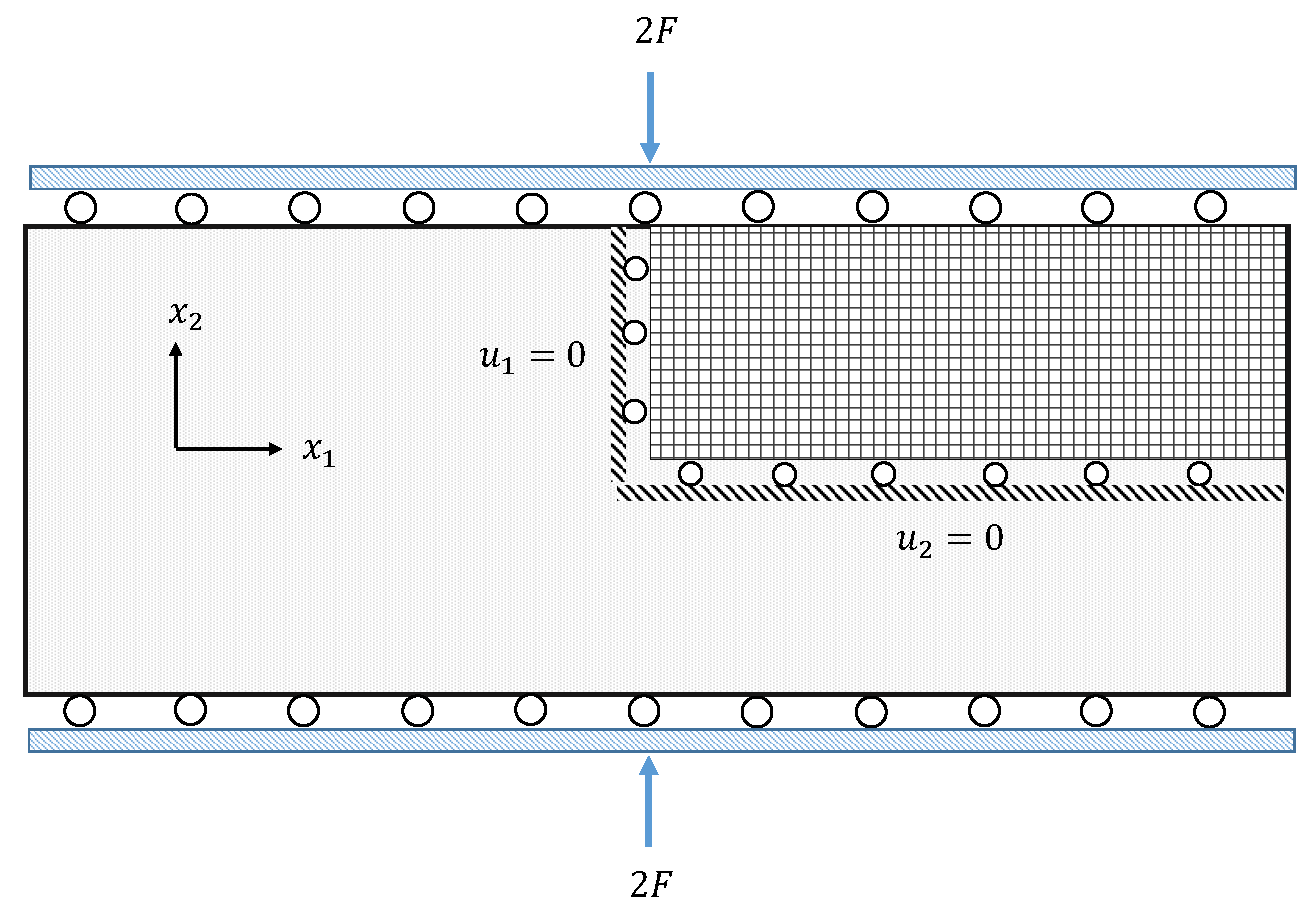
\includegraphics[width=0.8\textwidth]{MANDEL}
	\caption{Schematic view of Mandel's problem. An instantaneous compression force $2F$ is applied on the horizontal edges. Due to symmetry, only a quarter of the sample is modeled with proper boundary conditions.}
	\label{Fig:mandel}
\end{figure}
The material parameters for rock and fluid are given in Table \ref{Tab:Mandel_input}. Using our proposed algorithm in combination with the fixed-stress split method (see \cite{chukwudozie2016application, mikelic2013convergence}, which we have now also cited in the manuscript, see Section 3), we solved the numerical problem for $t_f=6$s in 600 equal time steps. Figure \ref{Fig:mandel_pressure} shows our numerical results and the analytical solution for pore pressure. Excellent agreement is observed. Figure \ref{Fig:mandel_snapshots} shows the pore pressure developed in the sample during consolidation.
\begin{table}[htbp]
	\centering
	\caption{Mandel's problem: Input parameters according to \cite{chukwudozie2016application}.}
	\begin{tabular}{l c c c}
		\hline 
		Parameters & symbol & unit& value \\
		\hline 
		Young's modulus & $E$ &MPa&  1\\
		Poisson's ratio & $\nu$ &$-$&  0.2\\
		Biot coefficient & $\alpha$ &$-$&  1.\\
		Permeability & $k_0$ &m$^2$&  1\\
		Viscosity &$\mu$ & MPa$\cdot$s &  1\\
		Length & $a$ & m &  2.5\\
		Height & $b$ & m &  1\\
		Load&$F$& MN& 2.5\\     
		Skempton coefficient &$B$& $-$& 1\\                    
		Drained Poisson's ratio&$\nu_u$& $-$&  0.5\\      
		Biot's modulus  & M & MPa & $\infty$ \\                                               
		\hline      
	\end{tabular}
	\label{Tab:Mandel_input}
\end{table}
\begin{figure}[htbp]
	\centering
	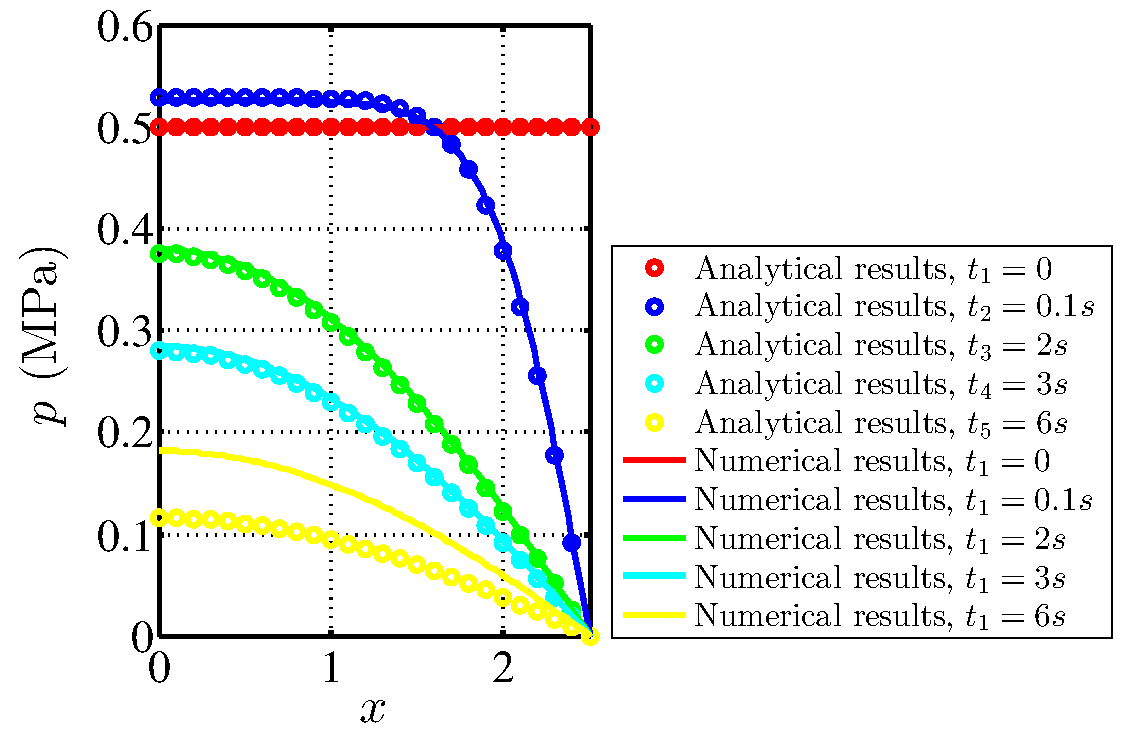
\includegraphics[width=0.8\textwidth]{mandel_pressure}
	\caption{Mandel's problem: change of pore pressure in time. Excellent agreement is observed with the analytical solution.}
	\label{Fig:mandel_pressure}
\end{figure}
\begin{figure}[htbp]
	\centering %
	\subfloat[]{
\includegraphics[width=80mm]{t9}\label{Fig:mandel_t_9}}
	\\
	\subfloat[]{
\includegraphics[width=80mm]{t199}\label{Fig:mandel_t_199}}
	\\
	\subfloat[]{
\includegraphics[width=80mm]{t299}\label{Fig:mandel_t_299}}
	\\
	\subfloat[]{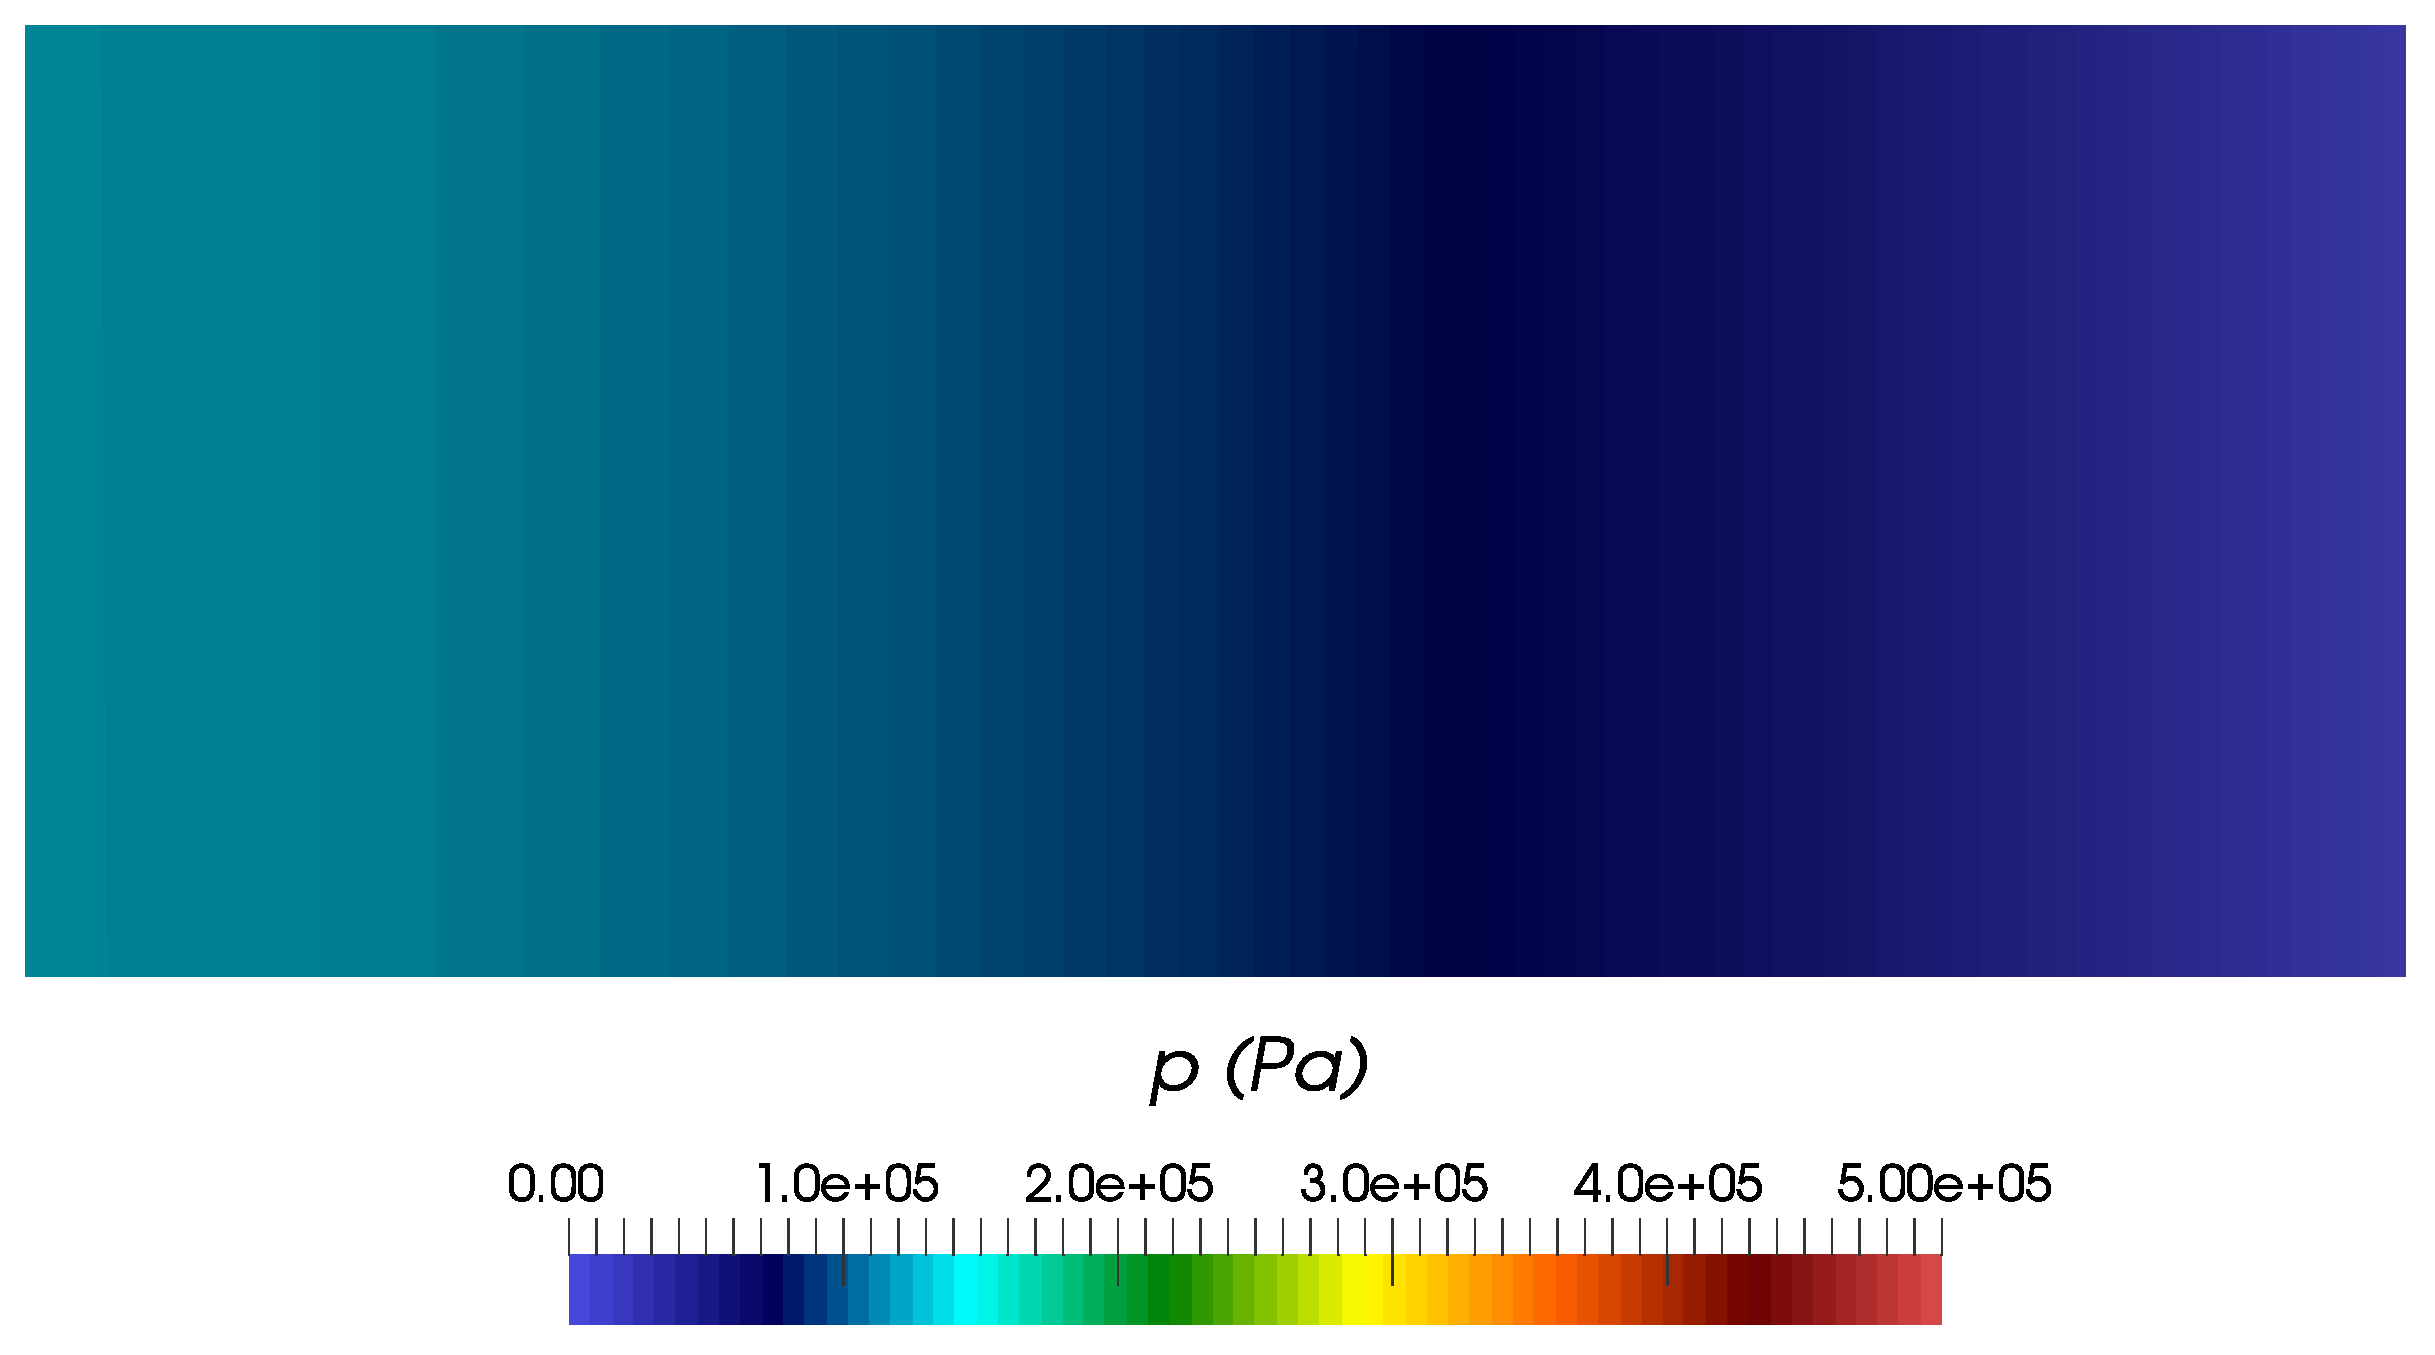
\includegraphics[width=80mm]{t599}\label{Fig:mandel_t_599}}
	\caption{Pressure profile at different stages (\ref{Fig:mandel_t_9}) $t=0.1s$, (\ref{Fig:mandel_t_199}) $t=2s$, (\ref{Fig:mandel_t_299}) $t=3s$, and (\ref{Fig:mandel_t_599}) $t=6s$). At very early stages, the pressure rises  rapidly in response to the instantaneous loading, then gradually decays to zero. %while drops until it nearly vanishes.
	}
	\label{Fig:mandel_snapshots}
\end{figure}
%A comment on Mandel's problem follows here.	
It is true that this problem is a typical poroelastic problem. However, it would somehow repeat our second verification example (see Section 4.2) where the porous flow is coupled with the porous medium's displacement. The example in Section 4.2 solved by Detourney and Cheng \cite{detournay1988poroelastic} has been used in a few works, e.g., \cite{wang2018influence, lu2013microcrack}, to verify the solution to the poroelastic response of a pressurized borehole. For these reasons, we preferred not to include Mandel's problem in the manuscript.